%!TEX root = ../dokumentation.tex

\chapter{Implementierung}

\section{BaklavaJS}

Eine der Anforderungen war es, das Modell visuell bearbeiten zu können. Dafür war es notwendig, einen Graph-Editor zu entwickeln. Ein solcher Editor erlaubt es, Knoten hinzuzufügen bzw. zu entfernen und sie miteinander zu verbinden.

Ein Knoten ist dabei wie eine mathematische Funktion: Er führt einen Algorithmus auf die Eingangsdaten aus und gibt die erzeugten Ausgangsdaten aus.

Visuell wird ein Knoten in BaklavaJS folgendermaßen dargestellt:

\begin{figure}[H]
    \centering
    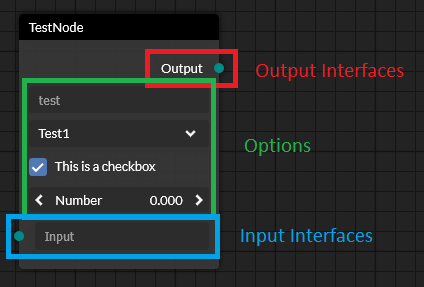
\includegraphics[width=.5\textwidth]{node_parts.png}
    \caption{Aufbau eines Knotens in BaklavaJS}
    \label{fig:nodeparts}
\end{figure}

Jeder Knoten besteht aus drei Teilen:
\begin{itemize}
    \item \textbf{Input Interfaces}: Die Eingangsschnittstellen eines Knotens werden benutzt, um Daten von anderen Knoten an diesen Knoten zu transferieren. Ist kein anderer Knoten verbunden, kann der Wert mittels eines Steuerelements auch direkt am Knoten eingestellt werden.
    \item \textbf{Options}: Hier können Werte eingestellt werden, die der Knoten für die Berechnung braucht, die aber beispielsweise zu komplex sind, um als Daten von anderen Knoten über Eingangsschnittstellen zu kommen.
    \item \textbf{Output Interfaces}: Die Ausgangsschnittstellen stellen das Ergebnis bereit, damit es von anderen Knoten benutzt werden kann.
\end{itemize}

\subsection{Ausführungsreihenfolge des Graphen}

\begin{figure}[H]
    \centering
    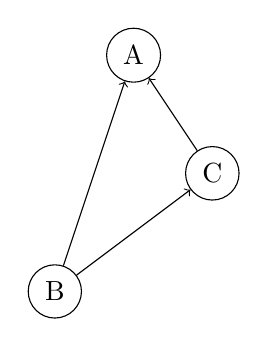
\begin{tikzpicture}
        \node[shape=circle,draw=black] (A) at (0,0) {A};
        \node[shape=circle,draw=black] (B) at (-1,-3) {B};
        \node[shape=circle,draw=black] (C) at (1,-1.5) {C};
        \path[->](B) edge node[left] {} (A);
        \path[->](B) edge node[left] {} (C);
        \path[->](C) edge node[left] {} (A);
    \end{tikzpicture}
    \caption{Beispielgraph}
    \label{fig:nodeExecutionOrder1}
\end{figure}

In Abbildung \ref{fig:nodeExecutionOrder1} ist ein Beispielgraph mit Knoten und Kanten zu sehen. Die Ausführungsreihenfolge der Knoten muss folgende Bedingungen erfüllen:
\begin{itemize}
    \item Jeder Knoten wird genau einmal ausgeführt
    \item Ein Knoten kann erst ausgeführt werden, wenn alle Knoten, die Kanten zu ihm haben, ausgeführt wurden
\end{itemize}

Um diese Anforderungen zu erfüllen, darf der Graph keine Zyklen enthalten. Mit folgendem Algorithmus kann die Ausführungsreihenfolge bestimmt werden:
\begin{enumerate}
    \item Adjazenzliste erstellen
    \item Baum aufbauen mit Zykluserkennung
    \item Breitensuche um die Ausführungsreihenfolge zu bestimmen 
\end{enumerate}

\begin{algorithm}[H]
    \caption{Baum aufbauen mit Zykluserkennung}
    \begin{algorithmic}[1]
        \Function{findDescendants}{treeNode, ancestors, adjacency}
            \ForAll{$c$ in $treeNode.children$}
                \If{$c$ in $ancestors$}
                    \State Cycle detected
                \EndIf
                \State $ancestors.push(c)$
                \State $c.children = findChildren(c)$
                \State \Call{findDescendants}{c, ancestors, adjacency}
                \State $ancestors.pop()$
            \EndFor
        \EndFunction
    \end{algorithmic}
\end{algorithm}

\begin{algorithm}[H]
    \caption{Breitensuche um die Ausführungsreihenfolge zu bestimmen}
    \begin{algorithmic}[1]
        \State $queue \gets \textbf{new} \ Queue()$
        \State $stack \gets \textbf{new} \ Stack()$
        \State $queue.push(root)$
        \While{\textbf{not} $queue.isEmpty()$}
            \State $current \gets queue.dequeue()$
            \ForAll{$c$ in $current.children$}
                \State $stack.push(c)$
                \State $queue.enqueue(c)$
            \EndFor
        \EndWhile
        \State $calculationOrder \gets \textbf{new} \ List()$
        \While{\textbf{not} $stack.isEmpty()$}
            \State $current \gets stack.pop()$
            \If{\textbf{not} $calculationOrder.contains(current)$}
                \State $calculationOrder.append(current)$
            \EndIf
        \EndWhile
    \end{algorithmic}
\end{algorithm}

Am Beispiel des Graphen in Abbildung \ref{fig:nodeExecutionOrder1} sieht der Algorithmus folgendermaßen aus:

\todo

\section{Random Sampling}

Mit Random Sampling ist eine Zufallsstichprobe gemeint bei der eine Stichprobe aus einer Grundgesamtheit $X$ mit $n$ Elementen gezogen wird. Seien die Elemente der Grundgesamheit $x_1,x_2,\dots,x_n-1,x_n$, dann unterliegt die Auswahl eines Elements $x \in M$ einem Auswahlverfahren, das angibt mit welcher Auftrittswahrscheinlichkeit $P(x)$ ein Element in die Stichprobe $N$ gelangen kann.
Es gelten die Bedingungen:
\begin{itemize}
    \item $P(x) > 0$ (Positivität)
    \item $\sum_{i=1}^{n}P(x_i)=1$ (Vollständigkeit)
\end{itemize}

Bei einer einfachen Zufallsstichprobe handelt es sich um die Auswahl einer Teilmenge einer statistischen Population, bei der jedes Element die gleiche Wahrscheinlichkeit $P(x)=\frac{1}{\lvert M \rvert}=\frac{1}{n}$ hat, ausgewählt zu werden. Zudem darf eine Ziehung aus einer Gesamtmenge nicht die nachfolgenden Ziehungen beeinflussen, weil sie unabhängig voneinander erfolgen müssen. Übertragen auf das typische Urnenexperiment der Stochastik, kommt es bei einer einfachen Zufallsstichprobe zu einer Ziehung mit Zurücklegen.

Für die Generation von Trainingsdaten ist das Random Sampling von großer Bedeutung, weil nur durch Einbeziehung einer Zufallskomponente neue Datensätze generiert werden können. Sollen beispielsweise zufällig ortspezfische Personendaten generiert werden, könnte die Herausforderung bestehen Daten von hunderten Personen aus nur vier Wohnorten zu generieren. Jeder Person soll dabei ein Wohnort zugewiesen werden, der zufällig bestimmt wird. Ist die Wahrscheinlichkeit für die Auswahl eines Wohnorts gleich groß, so ergibt sich eine einfache Zufallsstichprobe.
Oft genügt eine Gleichverteilung jedoch nicht, um eine Zufallsvariable zu modellieren, weil in der Realität andere Faktoren die Wahrscheinlichkeitsverteilung beeinflussen. Will man bezogen auf die Generation von Personendaten beispielsweise Größen generieren, wird eine Normal-, auch Gauß- oder Glockenverteilung benötigt.
Es kann auch sein, dass die Wahrscheinlichkeitsverteilung so spezifisch definiert ist, dass sie nicht mit einer einzigen Funktion dargestellt werden kann.

In den folgenden Kapiteln soll auf die genannten Fälle und deren Umsetzung eingegangen werden.

\subsection{Generation von gleichverteilten Zufallszahlen}

Für die einfache Zufallsstichprobe kann das Problem auf die Frage reduziert werden, wie eine gleichverteilte Zufallszahl in dem Intervall $I=[0;1]$ generiert werden kann. Diese Zufallszahl kann dann auf ein beliebiges Intervall transformiert werden. Sei $x_1$ eine gleichverteilte Zufallszahl im Intervall $I_1=[0;1]$ und seien $a$, $b$ Grenzen des Intervalls $I_2=[a;b]$, so ist die Zufallszahl $x_2$ im intervall $I_2$ bestimmt durch $x_2=x_1 \cdot b+a$. Durch das Runden auf die Einerstelle, können so diskrete Werte generiert werden.

Um gleichverteilte Zufallszahlen generieren zu können wird ein \ac{PRNG} verwendet.

Wie können random Zahlen generiert werden? 
- Theorie PRNG
- Beispielimplementierungen von PRNGs
- schlechte und gute PRNGs vergleichen

\subsection{Generation von nicht-gleichverteilten Zufallszahlen}

Warum brauchen wir auch nicht-verteilte Zufallswerte mit Beispielen?
- Normalverteilung (Größe), Exponentialverteilung (Bremsweg vs Geschwindigkeit)

\subsection{Generation von Zufallszahlen einer benutzerdefinierten Wahrscheinlichkeitsverteilung}

Was ist damit gemeint und warum brauchen wir benutzerdefinierte Zufallszahlen?
Wie ist das Problem bei benutzerdefinierten Wahrscheinlichkeitsverteilung und wie kann dies am einfachsten gelöst werden?
Der CustomRandom-Node teilt sich in drei verschiedene Komponenten: 1. UI, 2. Interpolation, 3. Berechnung

\subsubsection{Benutzerdefinierte Erstellung einer Wahrscheinlichkeitsverteilung}

--> Anzeige und benutzerdefinierte Erstellung einer Wahrscheinlichkeitsverteilung im Graph-Editor
- Chart.js, Canvas

\subsubsection{Inerpolation der erstellten Wahrscheinlichkeitsverteilung}

- Chart.js bietet out-of-the-box bereits Interpolationsmöglichkeiten an, jedoch gibt es keine geeignete Schnittstelle, um auf die Interpolationsdaten zuzugreifen, daher muss eigener Algorithmus implementiert werden

\subsubsection{Bestimmung der inversen kummulativen Wahrscheinlichkeitsverteilung}
--> Bestimmung der inversen kummulativen Wahrscheinlichkeitsverteilung
- Bestimmung der Integrierten Funktion
- Bestimmung der Inversen
- Sei x eine gleichverteilte reelle Zahl zwischen 0 und 1, so ist die custom-verteile Zahl bestimmt durch cdf-1(xmaxcdf)